% ============================================================
% DRAFT — §1.2 Inverse Trigonometric Functions
% stage ④ expansion toward ch01/brief_s12.md (direction layer, Ch1 full run).
% EXPERIMENT ARTIFACT — NOT for chapters/*.tex.
% % expansion: markers = additions beyond the manuscript seed (seed_s12.md).
% ③ decisions baked in:
%   (A) csc^{-1}/sec^{-1} ranges follow the MANUSCRIPT's non-standard
%       (differentiation-friendly) convention; ADD a caution flagging the
%       convention and the common alternative.
%   (B) ADD all three inverse self-graphs (arcsin/arccos/arctan), drawn as
%       reflections of the restricted forward graph across y=x (ROADMAP key
%       figure = restricted forward graphs, principal interval shaded).
%   (C) ADD a principal-interval trap example arcsin(sin(5pi/6)) = pi/6.
%   + sin^{-1} x != 1/sin x caution; one evaluation example each for arccos,
%     arctan; history/application skipped; inverse-trig DERIVATIVES forward-ref
%     to Ch3 only (manuscript gives only the "simpler differentiation" reason).
% Back-labels assumed as if integrated: sec:inverse-functions (§1.1),
%   prop:horizontal-line-test, fig:reflection-y-equals-x; forward: Ch3 derivatives.
% ============================================================

\section{Inverse Trigonometric Functions}\label{sec:inverse-trig-functions}

% expansion:intuition — section opener; reuse §1.1's horizontal line test as the obstruction
The machinery of \cref{sec:inverse-functions} applies only to one-to-one functions, and the trigonometric functions are the opposite of one-to-one: being periodic, each of them repeats every value infinitely often. A horizontal line drawn across the graph of \(\sin x\) meets it not twice but infinitely many times, so by the horizontal line test (\cref{prop:horizontal-line-test}) there is no inverse on the whole real line. The remedy is the domain-restriction idea previewed in \cref{sec:inverse-functions}: cut each trigonometric function down to a \emph{principal interval} on which it \emph{is} one-to-one, and invert it there.

\subsection{The inverse sine function}

On the interval \([-\pi/2, \pi/2]\) the sine function increases steadily from \(-1\) to \(1\), taking each value exactly once. Restricted to this principal interval, \(\sin\) is one-to-one and therefore has an inverse.

\begin{definition}\label{def:arcsin}\index{inverse sine function}\index{arcsin@$\arcsin$}
The \emph{inverse sine} (or \emph{arcsine}) function is the inverse of \(\sin x\) restricted to \([-\pi/2, \pi/2]\). Written \(\sin^{-1}\) or \(\arcsin\), it is defined by
\[
\sin^{-1} x = y \quad\Longleftrightarrow\quad \sin y = x, \qquad -\tfrac{\pi}{2} \le y \le \tfrac{\pi}{2}.
\]
Since \(\sin y\) ranges over \([-1, 1]\) as \(y\) ranges over \([-\pi/2, \pi/2]\), the domain of \(\sin^{-1}\) is \([-1, 1]\) and its range is \([-\pi/2, \pi/2]\).
\end{definition}

% expansion:caution — ROADMAP common pitfall: inverse vs reciprocal
\begin{caution}\index{inverse sine function!notation}
The notation \(\sin^{-1} x\) means the inverse sine of \(x\), \emph{not} the reciprocal \(1/\sin x\). When the reciprocal is intended, write \(1/\sin x\) or \(\csc x\). The name \(\arcsin x\) avoids the ambiguity entirely.
\end{caution}

% expansion:figure — restricted sine (principal interval shaded; ROADMAP key figure) AND arcsin as its reflection across y=x (③ fork B; manuscript draws only the restricted forward graph)
\begin{figure}[H]
\centering
\begin{tikzpicture}[scale=1.0]
  \fill[colorprimary!8] (-1.5708,-1.85) rectangle (1.5708,1.85);
  \draw[->] (-2.0,0) -- (2.0,0) node[right] {\(x\)};
  \draw[->] (0,-2.0) -- (0,2.0) node[above] {\(y\)};
  \draw[dashed] (-1.9,-1.9) -- (1.9,1.9) node[above right] {\(y = x\)};
  \draw[thick, colorprimary, domain=-1.5708:1.5708, smooth, samples=60]
        plot (\x, {sin(deg(\x))}) node[right] {\(\sin x\)};
  \draw[thick, colorcaution, domain=-1:1, smooth, samples=60]
        plot (\x, {rad(asin(\x))}) node[above left] {\(\arcsin x\)};
\end{tikzpicture}
\caption{The sine function restricted to the shaded principal interval \([-\pi/2, \pi/2]\) is one-to-one; \(\arcsin\) is its reflection across the line \(y = x\).}
\label{fig:inverse-sine}
\end{figure}

To evaluate an inverse sine, read the defining equivalence from right to left: find the angle in \([-\pi/2, \pi/2]\) whose sine is the given number.

\begin{workedexample}
\begin{example}\label{ex:arcsin-half}
Evaluate \(\sin^{-1}\!\bigl(\tfrac{1}{2}\bigr)\).
\end{example}

\begin{solution}
Set \(\sin^{-1}\!\bigl(\tfrac{1}{2}\bigr) = y\), so \(\sin y = \tfrac{1}{2}\) with \(-\pi/2 \le y \le \pi/2\). The angle in that range with sine \(\tfrac{1}{2}\) is \(y = \pi/6\). Hence \(\sin^{-1}\!\bigl(\tfrac{1}{2}\bigr) = \pi/6\).
\end{solution}
\end{workedexample}

Compositions of a trigonometric function with a \emph{different} inverse trigonometric function are handled by naming the inner angle and drawing a right triangle that realises it.

\begin{workedexample}
\begin{example}\label{ex:tan-arcsin}
Find \(\tan\!\bigl(\arcsin \tfrac{1}{3}\bigr)\).
\end{example}

\begin{solution}
Let \(\theta = \arcsin \tfrac{1}{3}\), so \(\sin \theta = \tfrac{1}{3}\) with \(\theta \in [-\pi/2, \pi/2]\). Draw a right triangle with opposite side \(1\) and hypotenuse \(3\); the adjacent side is \(\sqrt{3^{2} - 1^{2}} = 2\sqrt{2}\).
\begin{center}
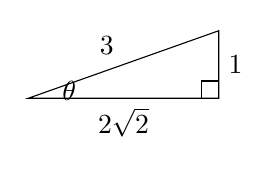
\begin{tikzpicture}[scale=1.1]
  \draw (0,0) -- (2.2,0) -- (2.2,0.78) -- cycle;
  \draw (2.0,0) -- (2.0,0.2) -- (2.2,0.2);
  \node[below] at (1.1,0) {\(2\sqrt{2}\)};
  \node[right] at (2.2,0.39) {\(1\)};
  \node[above left] at (1.1,0.39) {\(3\)};
  \node[right] at (0.28,0.08) {\(\theta\)};
\end{tikzpicture}
\end{center}
Then \(\tan \theta = \dfrac{\text{opposite}}{\text{adjacent}} = \dfrac{1}{2\sqrt{2}}\).
\end{solution}
\end{workedexample}

Reading \cref{def:arcsin} as a pair of cancellation equations (the inverse-function identities of \cref{sec:inverse-functions} specialised to \(\sin\)) records how \(\sin\) and \(\sin^{-1}\) undo each other --- but only on the principal interval.

\begin{proposition}[Inverse-sine cancellation]\label{prop:arcsin-cancellation}\index{inverse sine function!cancellation}
\[
\sin^{-1}(\sin x) = x \ \text{ for } -\tfrac{\pi}{2} \le x \le \tfrac{\pi}{2},
\qquad
\sin(\sin^{-1} x) = x \ \text{ for } -1 \le x \le 1.
\]
\end{proposition}

% expansion:caution — ROADMAP common pitfall: arcsin(sin x)=x only on the principal interval
\begin{caution}\index{inverse sine function!principal-interval restriction}
The identity \(\sin^{-1}(\sin x) = x\) holds \emph{only} for \(x\) in the principal interval \([-\pi/2, \pi/2]\). For other \(x\) the left side returns the principal angle with the same sine, which need not be \(x\).
\end{caution}

% expansion:example — principal-interval trap (③ fork C); manuscript states the identity but gives no out-of-range example
\begin{workedexample}
\begin{example}\label{ex:arcsin-sin-trap}
Evaluate \(\arcsin\!\bigl(\sin \tfrac{5\pi}{6}\bigr)\).
\end{example}

\begin{solution}
Here \(5\pi/6\) is \emph{not} in \([-\pi/2, \pi/2]\), so we may not simply cancel. First \(\sin \tfrac{5\pi}{6} = \tfrac{1}{2}\), and then \(\arcsin \tfrac{1}{2} = \pi/6\). Thus \(\arcsin\!\bigl(\sin \tfrac{5\pi}{6}\bigr) = \pi/6 \ne \tfrac{5\pi}{6}\): the inverse sine returns the principal angle \(\pi/6\), which shares its sine with \(5\pi/6\).
\end{solution}
\end{workedexample}

\subsection{The inverse cosine function}

The cosine function is not one-to-one on \([-\pi/2, \pi/2]\) (it is even), but on \([0, \pi]\) it decreases steadily from \(1\) to \(-1\) and so is one-to-one there. That interval is the principal interval for inverting cosine.

\begin{definition}\label{def:arccos}\index{inverse cosine function}\index{arccos@$\arccos$}
The \emph{inverse cosine} (or \emph{arccosine}) function is the inverse of \(\cos x\) restricted to \([0, \pi]\). Written \(\cos^{-1}\) or \(\arccos\), it is defined by
\[
\cos^{-1} x = y \quad\Longleftrightarrow\quad \cos y = x, \qquad 0 \le y \le \pi,
\]
with domain \([-1, 1]\) and range \([0, \pi]\).
\end{definition}

% expansion:figure — restricted cosine (principal interval shaded) and arccos as reflection across y=x (③ fork B)
\begin{figure}[H]
\centering
\begin{tikzpicture}[scale=0.95]
  \fill[colorprimary!8] (0,-1.4) rectangle (3.1416,3.1416);
  \draw[->] (-1.5,0) -- (3.5,0) node[right] {\(x\)};
  \draw[->] (0,-1.5) -- (0,3.5) node[above] {\(y\)};
  \draw[dashed] (-1.3,-1.3) -- (3.4,3.4) node[above right] {\(y = x\)};
  \draw[thick, colorprimary, domain=0:3.1416, smooth, samples=60]
        plot (\x, {cos(deg(\x))}) node[below right] {\(\cos x\)};
  \draw[thick, colorcaution, domain=-1:1, smooth, samples=60]
        plot (\x, {rad(acos(\x))}) node[above right] {\(\arccos x\)};
\end{tikzpicture}
\caption{The cosine function restricted to the shaded principal interval \([0, \pi]\) is one-to-one; \(\arccos\) is its reflection across the line \(y = x\).}
\label{fig:inverse-cosine}
\end{figure}

% expansion:example — small evaluation example for arccos (manuscript gives none)
\begin{workedexample}
\begin{example}\label{ex:arccos-half}
Evaluate \(\cos^{-1}\!\bigl(\tfrac{1}{2}\bigr)\).
\end{example}

\begin{solution}
We need the angle in \([0, \pi]\) with cosine \(\tfrac{1}{2}\); that angle is \(\pi/3\). Hence \(\cos^{-1}\!\bigl(\tfrac{1}{2}\bigr) = \pi/3\).
\end{solution}
\end{workedexample}

\subsection{The inverse tangent function}

On the open interval \((-\pi/2, \pi/2)\) the tangent function increases from \(-\infty\) to \(+\infty\), taking every real value exactly once. It is one-to-one there, and inverting it produces a function defined on the \emph{whole} real line.

\begin{definition}\label{def:arctan}\index{inverse tangent function}\index{arctan@$\arctan$}
The \emph{inverse tangent} (or \emph{arctangent}) function is the inverse of \(\tan x\) restricted to \((-\pi/2, \pi/2)\). Written \(\tan^{-1}\) or \(\arctan\), it is defined by
\[
\tan^{-1} x = y \quad\Longleftrightarrow\quad \tan y = x, \qquad -\tfrac{\pi}{2} < y < \tfrac{\pi}{2},
\]
with domain \((-\infty, \infty)\) and range \((-\pi/2, \pi/2)\).
\end{definition}

% expansion:figure — restricted tangent (principal interval shaded) and arctan as reflection across y=x (③ fork B)
\begin{figure}[H]
\centering
\begin{tikzpicture}[scale=0.85]
  \fill[colorprimary!8] (-1.5708,-3.2) rectangle (1.5708,3.2);
  \draw[->] (-3.4,0) -- (3.4,0) node[right] {\(x\)};
  \draw[->] (0,-3.4) -- (0,3.4) node[above] {\(y\)};
  \draw[dashed] (-3.2,-3.2) -- (3.2,3.2) node[above right] {\(y = x\)};
  \draw[thick, colorprimary, domain=-1.28:1.28, smooth, samples=80]
        plot (\x, {tan(deg(\x))}) node[right] {\(\tan x\)};
  \draw[thick, colorcaution, domain=-3.2:3.2, smooth, samples=80]
        plot (\x, {rad(atan(\x))}) node[right] {\(\arctan x\)};
  \draw[dotted] (-1.5708,-3.2) -- (-1.5708,3.2);
  \draw[dotted] (1.5708,-3.2) -- (1.5708,3.2);
\end{tikzpicture}
\caption{The tangent function restricted to the shaded principal interval \((-\pi/2, \pi/2)\) is one-to-one; \(\arctan\) is its reflection across \(y = x\), with horizontal asymptotes at \(\pm \pi/2\).}
\label{fig:inverse-tangent}
\end{figure}

A composition such as \(\cos(\tan^{-1} x)\) can be simplified to an algebraic expression, either with a Pythagorean identity or with a right triangle.

\begin{workedexample}
\begin{example}\label{ex:cos-arctan}
Simplify \(\cos(\tan^{-1} x)\).
\end{example}

\begin{solution}
Let \(y = \tan^{-1} x\), so \(\tan y = x\) with \(-\pi/2 < y < \pi/2\); we want \(\cos y\). From the identity \(1 + \tan^{2} y = \sec^{2} y\),
\[
\sec^{2} y = 1 + x^{2}, \qquad \sec y = \sqrt{1 + x^{2}},
\]
where we take the positive root because \(\sec y > 0\) on \((-\pi/2, \pi/2)\). Therefore
\[
\cos y = \frac{1}{\sec y} = \frac{1}{\sqrt{1 + x^{2}}}.
\]
This derivation holds for every real \(x\). For \(x \ge 0\) the same value reads off a reference triangle with opposite leg \(x\), adjacent leg \(1\), and hypotenuse \(\sqrt{1 + x^{2}}\):
\begin{center}
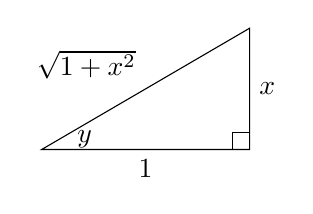
\begin{tikzpicture}[scale=1.1]
  \draw (0,0) -- (2.4,0) -- (2.4,1.4) -- cycle;
  \draw (2.2,0) -- (2.2,0.2) -- (2.4,0.2);
  \node[below] at (1.2,0) {\(1\)};
  \node[right] at (2.4,0.7) {\(x\)};
  \node[above left] at (1.2,0.7) {\(\sqrt{1 + x^{2}}\)};
  \node[right] at (0.3,0.12) {\(y\)};
\end{tikzpicture}
\end{center}
so that \(\cos y = \dfrac{\text{adjacent}}{\text{hypotenuse}} = \dfrac{1}{\sqrt{1 + x^{2}}}\), in agreement with the identity result for all real \(x\).
\end{solution}
\end{workedexample}

% expansion:example — small evaluation example for arctan (manuscript gives none)
\begin{workedexample}
\begin{example}\label{ex:arctan-one}
Evaluate \(\tan^{-1}(1)\).
\end{example}

\begin{solution}
The angle in \((-\pi/2, \pi/2)\) with tangent \(1\) is \(\pi/4\), so \(\tan^{-1}(1) = \pi/4\).
\end{solution}
\end{workedexample}

\subsection{The remaining inverse trigonometric functions}

The cosecant, secant, and cotangent are inverted on principal intervals in the same way, though they appear less often. Writing \(\arccsc\), \(\arcsec\), \(\arccot\) (equivalently \(\csc^{-1}\), \(\sec^{-1}\), \(\cot^{-1}\)) for the three inverses,\index{inverse cosecant function}\index{inverse secant function}\index{inverse cotangent function} each is one-to-one on the indicated set:
\[
\begin{aligned}
y = \arccsc x \ (\lvert x \rvert \ge 1) &\iff \csc y = x, \quad y \in (0, \tfrac{\pi}{2}] \cup (\pi, \tfrac{3\pi}{2}], \\
y = \arcsec x \ (\lvert x \rvert \ge 1) &\iff \sec y = x, \quad y \in [0, \tfrac{\pi}{2}) \cup [\pi, \tfrac{3\pi}{2}), \\
y = \arccot x \ (x \in \mathbb{R}) &\iff \cot y = x, \quad y \in (0, \pi).
\end{aligned}
\]

% expansion:caution — ③ fork A: the csc^{-1}/sec^{-1} ranges are a convention; flag the common alternative and the reason for this book's choice
\begin{caution}\index{inverse secant function!range convention}
The principal ranges chosen here for \(\sec^{-1}\) and \(\csc^{-1}\) are a \emph{convention} and differ between textbooks. Many books instead place the second branch of \(\sec^{-1}\) on \((\pi/2, \pi]\), giving range \([0, \pi/2) \cup (\pi/2, \pi]\). This book uses the branch on \([\pi, 3\pi/2)\) because it makes the differentiation formulas for \(\sec^{-1}\) and \(\csc^{-1}\) simpler (those derivative formulas are obtained in Chapter~3). When comparing with another source, check which convention it adopts.
\end{caution}

% expansion:summary — closing synthesis + forward pointer to §1.3 (limits)
With the six inverse trigonometric functions defined on their principal intervals, the chapter's algebraic machine --- running a rule backward --- is complete. The rest of Chapter~1 turns to its analytic counterpart: limits, the precise language for ``approaching without equalling'' that the next section begins.

% TODO: add \subsection*{Exercises} block for §1.2, following CONTENT_SPEC.md §14 and CONTENT_EXERCISES.md.
